\section{Solution}
\label{sec:compiler:solution}

We identify the sources of inadequacy w.r.t. assembly as violations of
three assumptions made by standard compilers: two on the registers and one on the stack.
We discuss why they 
cause problems with counterexamples and show how to semantically
handle them without changing the underlying language semantics.

\subsection{Assumptions on the Registers}
\label{sec:overview-semantics-register}
%
The two problematic assumptions on the registers are that
an invoked assembly function $(i)$ should
preserve the initial values of the callee-save registers, and $(ii)$
should not access the memory via the leftover pointer values remaining
in those registers that are not involved in passing meaningful information to the callee,
which we henceforth call \emph{\nip{}} registers.
%% in those registers, which we call \emph{non-passing} registers,
%% that are not involved in passing information to the callee.
%% the \emph{non-passing} registers (\ie those registers not involved
%% in passing information to the callee).
%% We discuss these two conventions together because it is nontrivial to find a
%% single model that enforces both conventions at the same time.
%% \jeehoon{I don't understand the last sentence..}
%% \jeehoon{``\nip{}'': how about ``opaque''?}

\begin{figure}[t]
\fbox{\begin{minipage}{.9pc}\mbox{}\\[15.25mm](a)\\[13.45mm]\mbox{}\end{minipage}}
\hspace*{-2.7mm}
\begin{minipage}{0.70\textwidth}
\begin{Verbatim}[frame=single]
int main()   {          main:
  int* x = malloc(8);     ...
  x[0] = 0;               *(%rbx) = 0;
  x[1] = 1;               *(%rbx + 4) = 1;
  f();               -->  f();
  out(x[0]);              out(*(%rbx));
  ...                     ...
}
\end{Verbatim}
\end{minipage}
$\mbox{}~\mathlarger{\mathlarger{\mathlarger{\mathlarger{\mathlarger{\llink}}}}}~\mbox{}$
\\
\vspace{3mm}
\\
\fbox{\begin{minipage}{.9pc}\mbox{}\\[10.50mm](b)\\[8.70mm]\mbox{}\end{minipage}}
\hspace*{-2.7mm}
\begin{minipage}{0.33\textwidth}
\begin{Verbatim}[frame=single]
f:
  if (g(%rbx))
    %rbx = %rbx + 4;
  else
    *(%rbx) = 1;

\end{Verbatim}
\end{minipage}
\caption{A counterexample showing the problem with the assumptions on the registers}
\label{fig:reg-convention}
\end{figure}

\myparagraph{Counterexamples}
%
The example in \Cref{fig:reg-convention} shows how violations of the two
assumptions can invalidate correct compiler translations.
%% \jeehoon{I think counterexample should go to the problems section.}
%
The code in the left box~(a) shows a standard translation of C code into assembly
(written in pseudocode) performed by mainstream compilers like GCC and LLVM, where the accesses to
the array \texttt{x} are translated into accesses via the register
\texttt{\%rbx} assuming that \texttt{\%rbx} is set to contain the
address of \texttt{x}. An important point here is that the compiler
assumes that $(i)$ the value of \texttt{\%rbx} is unchanged across
the function call \texttt{f()} since it is a callee-save register,
and also $(ii)$ the values in the array pointed to by \texttt{\%rbx} are
unchanged across \texttt{f()} since the array's addresses do not escape
except via \nip{} registers like \texttt{\%rbx}.
Therefore, the compiler expects that \texttt{out(*(\%rbx))} in the target code
correctly outputs \texttt{0}.

The right box~(b) presents an example of handwritten assembly
(written in pseudocode) for function \texttt{f} that violates the
above two assumptions of the compiler. The code either increments
\texttt{\%rbx} by \texttt{4} or writes \texttt{1} to \texttt{*(\%rbx)}
depending on the result of call to \texttt{g}.  Now if we link the assembly
code in (a) and that in (b) together, one can easily see that
\texttt{out(*(\%rbx))} incorrectly outputs~\texttt{1} instead
of \texttt{0} in either case: in the former case, \texttt{\%rbx}
points to the second element of the array~\texttt{x}, which contains
\texttt{1}; in the latter case, the value of \texttt{*(\%rbx)} is
directly updated to \texttt{1}. Therefore, it makes sense to
define those illegal behaviors of (b) as undefined behavior~(UB).

\myparagraph{Our Model}
\label{sec:compiler:solution:model}
%
We present our model making the illegal behaviors UBs
in stages, explaining at each stage why naive models do not work.
%% \jeehoon{What's the difference between ``stage'' and ``state''?}
%% \jeehoon{We have ``Our Solution'' paragraph inside ``Our Solution'' section. How about moving
%%   counterexample to the problems section, and giving a paragraph to each stage?}

First, in order to enforce the preservation of callee-save register
values, we store the initial values of the callee-save registers at
the \texttt{init-core} step of assembly modules; and check, at the
\texttt{halted} step, whether the final values of those registers are
equal to the stored initial values and if not, raise UB.  Here, the
question is, when a new core with a fresh register file is pushed into the core stack,
what values should be set as initial values of the \nip{}
registers including all of the callee-save registers.  Since the
registers may contain arbitrary values in the physical assembly
semantics, a natural choice would be to initially set them to contain
the \texttt{undef} value, which is an abstract value representing all
possible values. Indeed, this is the choice of \ccc{}.  However, there
is a serious problem. Since, for instance, \texttt{undef + 4} results
in \texttt{undef}, checking whether the final values of callee-save
registers are equal to the initial values, \ie \texttt{undef}, is
not sufficient. Specifically, the assembly code in (b) above
does not raise UB in this new semantics in case \texttt{g(\%rbx)} returns \texttt{1}
because the initial and final values of \texttt{\%rbx}
are both \texttt{undef} and thus equal
even though the callee-save register \texttt{\%rbx} is incremented
by \texttt{4} in the physical semantics.

Second, another natural solution would be to initially set the
\nip{} registers to nondeterministically contain arbitrary
values including \texttt{undef}. Though this model is more flexible,
it still has a problem. For instance, in the above example, to
simulate the physical behaviors of the assembly function \texttt{f} in
interaction semantics, one can set the initial value of \texttt{\%rbx} to
be either $(i)$ \texttt{undef} (\ie a more abstract value than the physical one), or
$(ii)$ a pointer to the array \texttt{x} (\ie a value equivalent to the physical one):
other values cannot be used since they are not refined by the value of \texttt{\%rbx} in the target,
which is required since the value is passed to an unknown function~\texttt{g}.
In the former case, if
\texttt{g(\%rbx)} returns \texttt{1}, we have the same problem with
callee-save checking as shown above.  In the latter case, if
\texttt{g(\%rbx)} returns \texttt{0}, the function \texttt{f}
successfully updates the array~\texttt{x} thereby invaliding the
translation in (a) as illustrated above.

We solve this problem by further revising the second model:
nondeterministically allocating an arbitrary number of \emph{junk
  blocks} (\ie blocks of size zero) and then initializing the
\nip{} registers with arbitrary non-pointer values or
\emph{junk pointers} (\ie pointers to the junk blocks).  Then we can
simulate the physical behaviors by initializing each register $r$
$(i)$ with the same non-pointer value if the physical value of $r$ is
a non-pointer value; and $(ii)$ otherwise with a fresh junk pointer.
The high-level idea is that, like \texttt{undef}, a junk pointer is
more abstract (\ie causing more UBs) than any pointer but, unlike
\texttt{undef}, sufficiently distinguishable. For instance,
in the previous example, if \texttt{g(\%rbx)} returns \texttt{1},
the initial and final values of \texttt{\%rbx} (\ie $p$ and $p+4$ for a junk pointer $p$)
are distinguished thereby raising UB by the callee-save checking;
if \texttt{g(\%rbx)} returns \texttt{0},
the memory access \texttt{*(\%rbx) = 1} raises UB because \texttt{\%rbx}
points to a junk block of size zero.

Finally, note that introducing nondeterminism as above is not a
showstopper thanks to the mixed simulation, as discussed in
\Cref{sec:overview-verification:mixedsim}: we can do forward
simulation everywhere except for the \texttt{init\_core} step of
assembly modules, where we should do backward simulation.

\subsection{Assumptions on the Stack}
\label{sec:overview-semantics-memory}
%
The problematic assumption on the stack is that the
\emph{outgoing arguments area} of a caller's stack (\ie where overflowing function
arguments are stored) should be fully \emph{owned} by the callee. In
other words, the callee can assume that the arguments area is never
modified by others unless its addresses are revealed to the public by
the callee itself.

\begin{figure}[t]
\fbox{\begin{minipage}{.9pc}\mbox{}\\[10.45mm](a)\\[8.65mm]\mbox{}\end{minipage}}
\hspace*{-1.9mm}
\begin{minipage}{0.255\textwidth}
  \begin{Verbatim}[frame=single]
main:
  ...  
  leak = %rsp;
  f(..., 0);
g:
  *leak = 1;
  \end{Verbatim}
\end{minipage}
$\mbox{}~\mathlarger{\mathlarger{\mathlarger{\mathlarger{\mathlarger{\llink}}}}}~\mbox{}$
\fbox{\begin{minipage}{.9pc}\mbox{}\\[10.45mm](b)\\[8.65mm]\mbox{}\end{minipage}}
\hspace*{-1.9mm}
\begin{minipage}{0.695\textwidth}
  \begin{Verbatim}[frame=single]
void f(..., int64_t x)       f:
{                              ...
  out(x);                      out(*(%rax));
  g();                  -->    g();
  out(x);                      out(*(%rax));
}                              ...
  \end{Verbatim}
\end{minipage}
\\[1mm]
\fbox{\begin{minipage}{.9pc}\mbox{}\\[15.90mm](c)\\[15.10mm]\mbox{}\end{minipage}}
\hspace*{-2.7mm}
\begin{minipage}{.95\textwidth}
\fbox{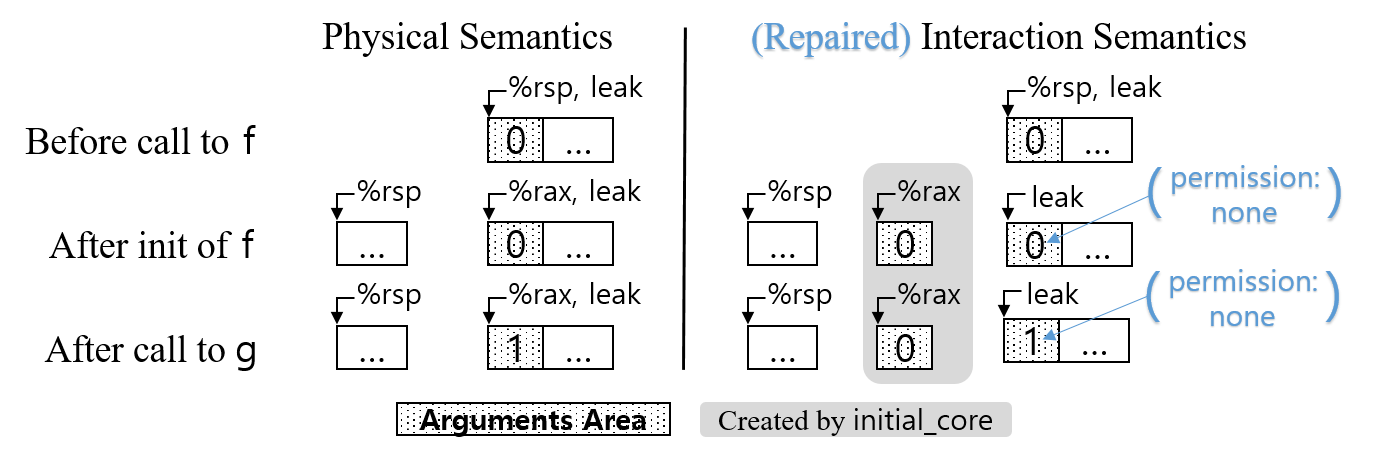
\includegraphics[width=.983\textwidth]{images/ex-stack.png}}
\end{minipage}
%% \fbox{\begin{minipage}{.8pc}\mbox{}\\[4.53mm](c)\\[3.73mm]\mbox{}\end{minipage}}
%% \hspace*{-1.9mm}
%% \begin{minipage}{.95\textwidth}
%%   \begin{Verbatim}[frame=single]
%%                      Physical Semantics         Interaction Semantics
%%                             %rsp           |                  %rsp       
%% Before call to f:           [=0=| ... ]    |                  [=0=| ... ]
%%                     %rsp    %rax           |    %rsp    %rax             
%%  After init of f:   [ ... ] [=0=| ... ]    |    [ ... ] [=0=] [=0=| ... ]
%%                     %rsp    %rax           |    %rsp    %rax             
%%  After call to g:   [ ... ] [=1=| ... ]    |    [ ... ] [=0=] [=1=| ... ]
%%   \end{Verbatim}
%% \end{minipage}
\caption{A counterexample showing the problem with the assumption on the stack}
\label{fig:stack-convention}
\end{figure}

\myparagraph{Counterexamples}
%
The example in \Cref{fig:stack-convention} shows how violations of the assumption
can invalidate correct compiler translations.
%
The box~(a) shows handwritten assembly code implementing two functions
\texttt{main} and \texttt{g}; the box~(b) shows a standard translation
of C code into assembly essentially performed by \texttt{gcc -O0}; and
the left-hand side (LHS) of the box~(c) depicts the shape of the stack
during execution in the physical semantics.
The function \texttt{main} stores the address of the
outgoing arguments area (\ie \texttt{\%rsp} as depicted in LHS of (c))
in the global variable \texttt{leak} and invokes the function
\texttt{f}, where the last argument \texttt{0} is stored in the
arguments area of the stack. Then the function \texttt{f} makes three
function calls, \texttt{out(x)}, \texttt{g()} and \texttt{out(x)},
where the argument \texttt{x} is directly read from the arguments area
pointed to by \texttt{\%rax} in the assembly, as depicted in LHS of
(c), and \texttt{out(x)} outputs the read value.  Finally, the
function \texttt{g} updates the arguments area pointed to by
\texttt{leak} with~\texttt{1}, as depicted in LHS of (c), between the
two function calls \texttt{out(x)}.

An important point here is that the compiler assumes that the
arguments area (\ie \texttt{\%rax}) is unchanged across the
function call \texttt{g()} since it is fully owned by \texttt{f}.
Therefore, the compiler expects that both calls
\texttt{out(*(\%rax))} in the target code correctly output
\texttt{0}. However, since the function \texttt{g} updates the
arguments area with \texttt{1} via \texttt{leak}, the two calls
incorrectly output \texttt{0} and~\texttt{1}.
We confirmed this incorrectness by
compiling \texttt{f} with \texttt{gcc -O2}, which
eliminates the second load \texttt{*(\%rax)} by propagating
the result of the first load across \texttt{g()}
thereby outputting \texttt{0} twice.

\myparagraph{Our Model}
%
In order to solve the problem, we have to distinguish accesses to the
arguments area via the caller from those via the callee and define the
former as UB. Though making such distinction is difficult in the
physical semantics, fortunately it is already made in interaction
semantics due to the language-independent design. For example, consider
the interaction semantics of the above example, depicted in the
right-hand-side (RHS) of \Cref{fig:stack-convention}~(c).  The
difference is that when the assembly function \texttt{f} is invoked,
the initialization process (\ie \texttt{init\_core}) of the module
semantics newly constructs the arguments area of the stack from the
given logical arguments in order to make an environment needed to
execute the assembly function \texttt{f}. This is essentially needed
because the caller may not be an assembly module so that it may not
have its own stack at all.  Then the callee sees the new arguments
area created by \texttt{init\_core} while the caller (in assembly)
sees the original arguments area.

Although the original interaction semantics does not prevent access to
the arguments area via the caller, we can easily fix it.
%% Now we can easily repair the original interaction semantics to make
%% those accesses to the arguments area via the caller as UB during the
%% lifetime of the callee.
We simply $(i)$ turn off the access
permission of the original arguments area in the \texttt{at\_external}
step of the caller module, and $(ii)$ turn it back on in the
\texttt{after\_external} step. Note that the notion of permission
%% is already an existing feature of
already exists in the \cc{} semantics, so that we do not
need to strengthen it. In the above example again,
the update by \texttt{g} will raise UB since the original argument area pointed
to by \texttt{leak} has no access permission.


\subsection{Mixed Simulation}
\label{sec:overview-verification:mixedsim}

While the target language of \cc{} is deterministic (more precisely,
the source is receptive and the target is determinate) thereby mostly
using forward simulations, the repaired interaction semantics of
\ccm{} is inherently nondeterministic to handle illegal interference from assembly modules
%% enforce the assembly calling conventions
(\Cref{sec:compiler:solution:model}) thus preventing the
use of forward simulation.
%% While it is theoretically possible to convert the \cc{}
%% verification from forward to backward simulations, it would incur a
%% significant cost since a compiler pass typically compiles a single
%% instruction in the source down to several instructions in the target.
%% %% due to the nature of source and target languages and the size of verification.
%% For this reason, determinism
%% has been considered ``instrumental for the simulation proofs of the compiler passes and its absence
%% is a show stopper''~\cite{besson:intptr}.
% Extending \cc{}'s semantics with such nondeterministic features can potentially cause significant
% overhead, as it invalidates forward simulation and enforces one to use backward simulation, which
% effectively means one should re-establish simulation proof from the scratch.  In literature, it is
% even said that

In order to recover the ability to use forward simulation in the occasional presence of nondeterminism,
we adopt the idea of \emph{mixed (forward-backward) simulation} from \cite{neis:pilsner}.
%% To embrace nondeterminism with low verification cost, we develop more general simulations, called
%% \emph{mixed simulations}, that (mostly) allow forward reasoning in the (occasional) presence of
%% nondeterminism.
The key observation is that
the requirement for using forward simulations (\ie determinism of the target) is a per-state property,
not a per-language property: as long as a particular target machine state is \emph{locally deterministic} (\ie its next state is unique),
one can do forward simulation at that state.
%% conversion from backward to forward simulations
%% requires only the current target \emph{machine state}, not the entire target \emph{language}, to be
%% deterministic.
Based on this observation, mixed simulations selectively allow forward
simulation when the target is locally deterministic, in addition to
the default backward simulation.
%% for each pair of related machine states, we allow the verifier to
%% \emph{choose} to perform either forward or backward reasoning, requiring that forward reasoning is
%% used only for locally deterministic target machine states.
%
Specifically, we say that a relation $R$ is a (closed) mixed simulation if
for all $(\mssrc, \mstgt) \in R$,
%% \makebox[\linewidth]{\makebox[1.2\linewidth]{
%% \begin{minipage}{1.2\linewidth}
\begin{enumerate}
\item
  $\forall e, \mstgt',~ \mstgt \estep{e} \mstgt' \implies {} $ \\
  $ \exists \mssrc',~ \mssrc \estep{\tau}^{\raisebox{-1mm}{\scriptsize$\ast$}} \estep{e}\estep{\tau}^{\raisebox{-1mm}{\scriptsize$\ast$}} \mssrc' \land (\mssrc', \mstgt') \in R$; or
\item
  $\forall e, \mssrc',~ \mssrc \estep{e} \mssrc' \implies {} $ \\
  $ \exists \mstgt',~ \mstgt \eustep{\tau}^{\raisebox{-1mm}{\scriptsize$\ast$}} \eustep{e}\eustep{\tau}^{\raisebox{-1mm}{\scriptsize$\ast$}} \mstgt' \land (\mssrc', \mstgt') \in R$\\
\end{enumerate}
%% \end{minipage}
%% }}
where $\ms \eustep{e} \ms'$ denotes that $\ms$ is locally deterministic and $\ms \estep{e} \ms'$.

\Cref{fig:mixedsim} visualizes this formulation of mixed simulation, where
%% presents an example of mixed simulations, where $R$ is a simulation relation; red and blue circle represent source and
%% target machine states, respectively;
solid and dotted arrows represent universally and existentially
quantified steps, respectively, and double circles represent locally
deterministic target states. In this figure,
since the first three target machine states are deterministic,
we can do forward simulation as shown in the figure;
then, since the following target state is nondeterministic,
we should do backward simulation as shown in the figure.
%% the first three target machine states are deterministic.  The
%% first three target steps are deterministic and reasoned in a forward manner (from source to target),
%% and the last target step is nondeterministic and reasoned in a backward manner (from target to
%% source).  Later, those part of simulations that are reasoned in a forward manner is converted to
%% backward reasoning, thereby proving backward simulation and thus behavior refinement.

Note that the repaired interaction semantics is nondeterministic only
at the initial step of a module invocation, so that we can do
forward simulation everywhere else using mixed simulations.

In order to support \cc{}'s condition for forward simulation,
we also add the following to the above formulation of mixed simulation:
\begin{enumerate}[resume]
\item or, $\mssrc$ is receptive and\\
  $\forall e, \mssrc',~ \mssrc \estep{e} \mssrc' \implies {} $ \\
  $ \exists \mstgt',~ \mstgt \exstep{\tau}^{\raisebox{-1mm}{\scriptsize$\ast$}} \exstep{e}\exstep{\tau}^{\raisebox{-1mm}{\scriptsize$\ast$}} \mstgt' \land (\mssrc', \mstgt') \in R$\\
  where $\ms \exstep{e} \ms'$ denotes that $\ms$ is locally determinate and $\ms \estep{e} \ms'$.
\end{enumerate}
Also we apply this mechanism of mixed simulation to our open simulations.

\begin{figure}[t]%% {0.43\textwidth}
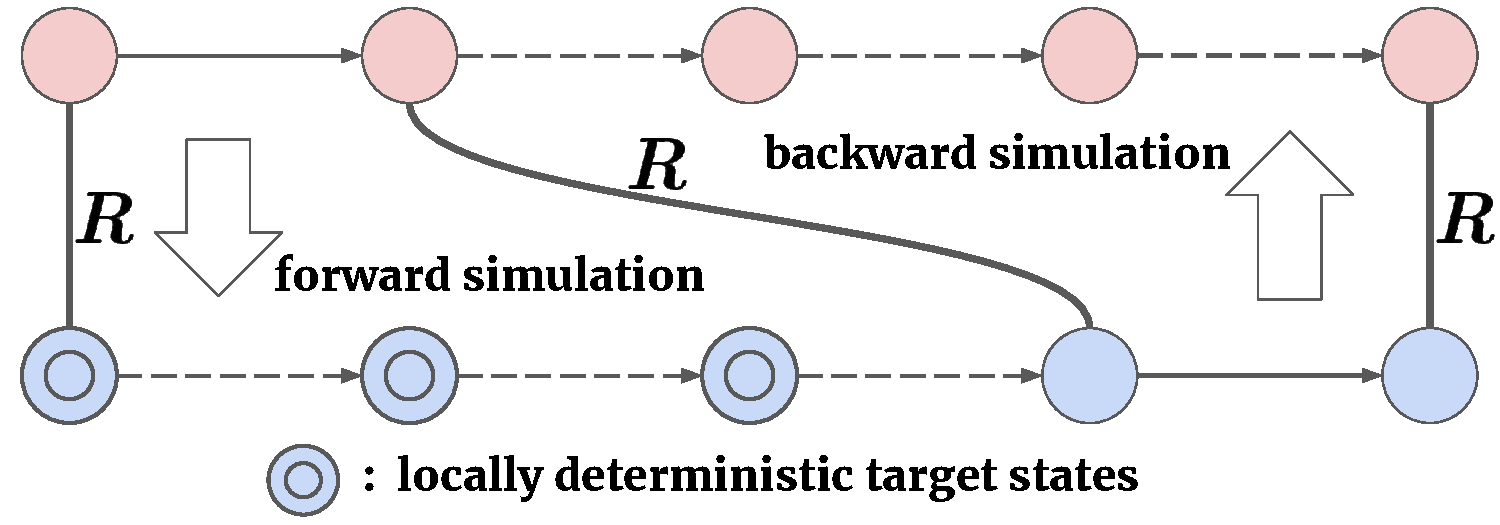
\includegraphics[width=0.7\textwidth]{images/mixed-sim-bold.pdf}
%% 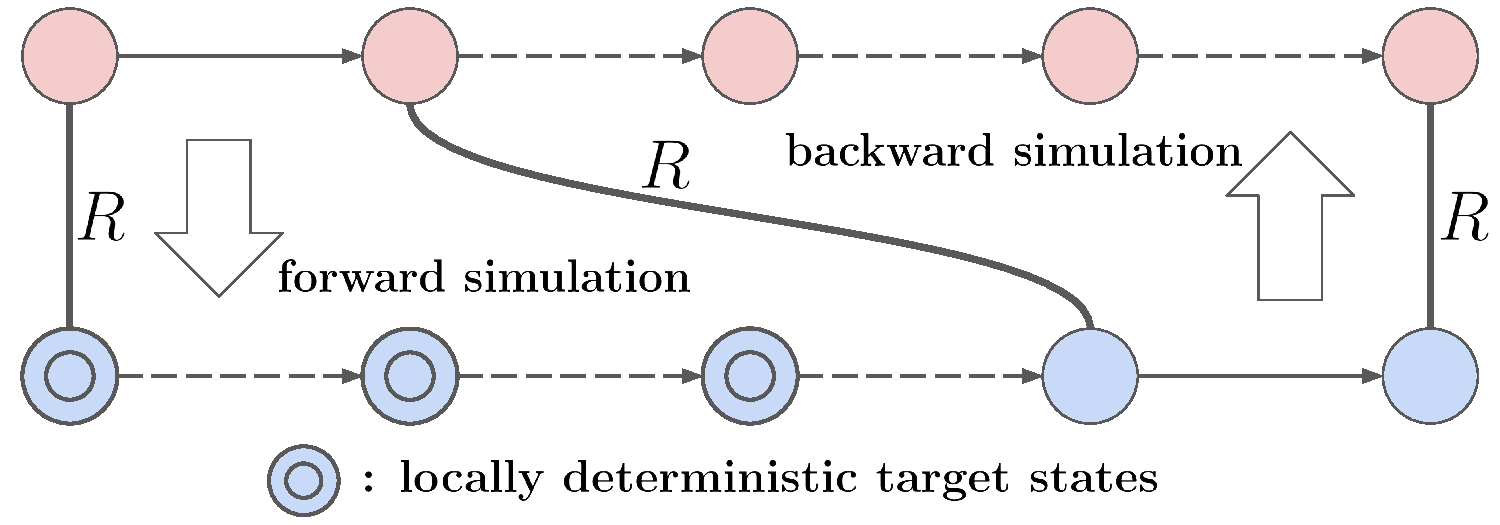
\includegraphics[width=0.7\textwidth]{images/mixed-sim.pdf}
\caption{A visualized example of mixed simulations}
\label{fig:mixedsim}
\end{figure}
